% vim: set tw=78 aw:
\documentclass{beamer}

\usepackage[utf8x]{inputenc} % diacritice
\usepackage[romanian]{babel}
\usepackage{color}			 % highlight
\usepackage{alltt}			 % highlight
\usepackage{code/highlight}	 % highlight
\usepackage{hyperref}        % folositi \url{http://...}
% sau \href{http://...}{Nume Link}
\mode<presentation>
\usetheme{CDL}

% Titlul nu foloseşte Unicode pentru că e o problemă căreia nu i-am dat de
% cap.
\title[Documentatia]{Documentatia}
\subtitle{CDL - Cursul 4}
\institute[ROSEdu]{ROSEdu}
\author[Adrian|Victor]{Victor Cărbune - Adrian Scoică\\(\small victor@rosedu.org - adrian.sc@rosedu.org)}

\begin{document}

% Slide-urile cu mai multe părţi sunt marcate cu textul (cont.)
\setbeamertemplate{frametitle continuation}[from second]
% Arătăm numărul frame-ului
\setbeamertemplate{footline}[frame number]

\frame{\titlepage}

\begin{frame}
\tableofcontents
\end{frame}

% NB: Secţiunile nu sunt marcate vizual, ci doar apar în cuprins.
\section{Introducere}

\begin{frame}{Documentația software}
	Ce este?
	\pause
	\begin{itemize}
		\item Text 
		\item Tutoriale
		\item Metainformații 
	\end{itemize} 
	... care însoțesc un produs software. \pause \\
	Pe cine vizează?
	\pause
	\begin{itemize}
		\item Proiectanți (Requirements, API)
		\item Dezvoltatori (API, SDK)
		\item Utilizatori (Manuale, Tutoriale)
	\end{itemize}
	
\end{frame}

\begin{frame}{The ugly truth}
\begin{center}
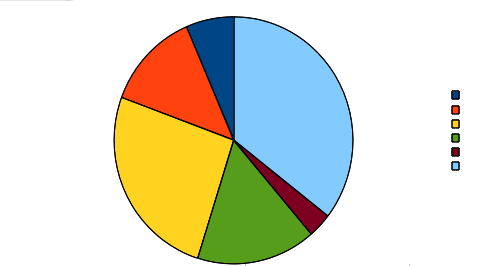
\includegraphics[height=5.5cm, width=11cm]{Step1.png}
\end{center}
\end{frame}

\begin{frame}{The ugly truth}
\begin{center}
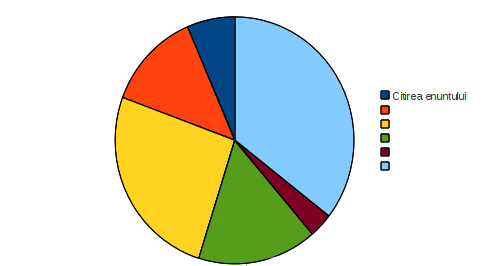
\includegraphics[height=5.5cm, width=11cm]{Step2.png}
\end{center}
\end{frame}

\begin{frame}{The ugly truth}
\begin{center}
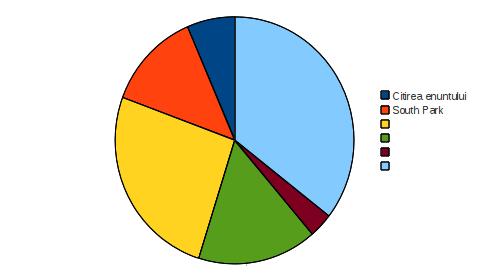
\includegraphics[height=5.5cm, width=11cm]{Step3.png}
\end{center}
\end{frame}

\begin{frame}{The ugly truth}
\begin{center}
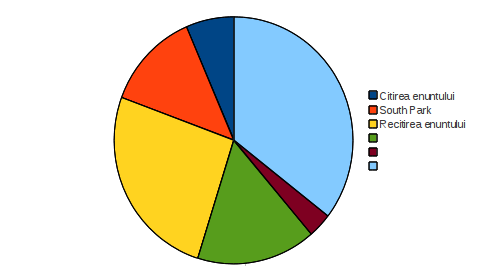
\includegraphics[height=5.5cm, width=11cm]{Step4.png}
\end{center}
\end{frame}

\begin{frame}{The ugly truth}
\begin{center}
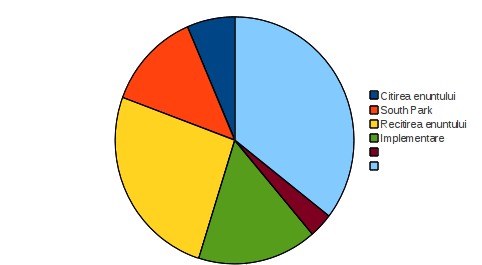
\includegraphics[height=5.5cm, width=11cm]{Step5.png}
\end{center}
\end{frame}

\begin{frame}{The ugly truth}
\begin{center}
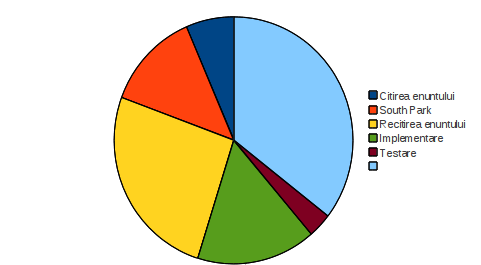
\includegraphics[height=5.5cm, width=11cm]{Step6.png}
\end{center}
\end{frame}

\begin{frame}{The ugly truth}
\begin{center}
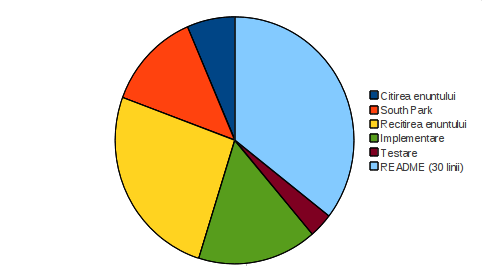
\includegraphics[height=5.5cm, width=11cm]{Step7.png}
\end{center}
\end{frame}

\begin{frame}{The ugly truth}
	Programatorii detestă să scrie documentație.
	\pause
	\begin{itemize}
		\item "Pentru că {\bf pare} timp mort"
		\pause
		\item "Pentru că {\bf PCTTOR\_BK\_TAG\_OP\_CLCL} este un nume de constanta sugestiv"
		\pause
		\item "Pentru că oricum este evident ce face {\bf int prior\_load(const std::priority\_queue$<$SCRTok::Lexem, std::vector$<$SCRTok::Lexem$>$, std::greater$<$SCRTok::Lexem$>$ $>$\& lex);}
		\pause
		\item "Pentru că oricum o să fac modificări mai târziu"
		\pause
	\end{itemize}
\end{frame}

\begin{frame}{Consecințele}
  \begin{itemize}
  \pause
  \item Codul este greu de refolosit, înțeles și modularizat
  \pause
  \item Devine un coșmar să încerci să adaugi funcționalități sau să repari bug-uri
  \pause
  \item Ceilalți programatori evită codul
  \end{itemize}
  \pause
  ... și în cele din urmă, proiectul moare.
\end{frame}

\section{Comentariile}

\section{Doxygen}

\section{pydoc}

\begin{frame}{Ce este pydoc?}
  \begin{itemize}
  \item Modul disponibil în limbajul Python
  \pause
  \item Generator de documentație în format Text / HTML pentru un modul Python
  (echivalent man pentru Unix)
  \pause
    \begin{itemize}
    \item pydoc sys
    \pause
    \item pydoc sys -w
    \end{itemize}
  \pause
  \item Server pentru documentație
    \begin{itemize}
      \item pydoc -p 80
    \end{itemize}
  \pause
  \item Căutari de cuvinte cheie
    \begin{itemize}
      \item pydoc -k "word"
    \end{itemize}
  \end{itemize}
\end{frame}

\begin{frame}{Cum scriem cod pentru a putea folosi pydoc?}
  \begin{itemize}
  \item Scrieți un modul test.py, care conține o clasă oarecare
  \item Rulați pydoc ./test.py
  \item Adăugați descriere la nivel de modul, clasa, metode
  \item Declarați global mai multe variabile / funcții
  \item Observați ce secțiuni s-au adăugat / modificat
  \end{itemize}
\end{frame}

\begin{frame}{Lab}
  \begin{itemize}
  \item Instalați Eclipse
  \pause
  \item Instalați CDT
		\begin{itemize} 
		\pause
	  \item Help ... Install New Software
  	\pause
	  \item Available Software ... Add Site
  	\item http://download.eclipse.org/tools/cdt/releases/galileo
  	\end{itemize}
  \item Creați un proiect C++ nou (HelloWorld)
  \end{itemize}
\end{frame}

\section{Resurse}

\begin{frame}{Resurse}
  \begin{itemize}
  \item http://www.eclipse.org
  \pause
  \item http://www.eclipseplugincentral.org  
  \pause
  \vspace{10mm}
  \item Întrebări?
  \end{itemize}
\end{frame}

\begin{frame}{}
\end{frame}

\end{document}
